\documentclass[main.tex]{subfiles}
\begin{document}


\section{Dirac Monopoles}\label{sect:Dirac}
In 1931 Dirac showed that postulating the existence of a magnetic charge, we can provide a theoretical explanation for the quantization of the electric charge \cite{Dirac}. 
In this section we will recover the basic ideas exposed in Dirac's paper and show how they were generalised to a particle with both charges, called \emph{dyon}, by Schwinger in 1966 \cite{S:dyon} and Zwanziger in 1968 \cite{Z:dyon}.

%To date no experiment has shown the existence of magnetic monopoles, but classical electromagnetic theory admits their existence in its gauge formulation \cite{Dirac}.
%This follows naturally from Maxwell equations' duality: monopoles are interesting solutions in a space with nontrivial topology, since from topological arguments one can derive the quantization of magnetic and electric charge.

\subsection{Magnetic Monopole and Electromagnetic Duality}

The electromagnetic tensor $F^{\mu \nu}$, where both electric and magnetic fields are encoded:
%
\begin{equation}
E^i=F^{0i} \qquad \qquad B^i=\epsilon^{ijk}F^{jk}\,,
\end{equation}
%
is an antisymmetric tensor and can be written as a 2-form (see appendix \ref{sec:differential-forms}): 
%
\begin{equation}
F = \frac{1}{2} F_{\mu\nu}\dd{x^\mu} \wedge \dd{x^\nu}
\,.
\end{equation}
%
It obeys Maxwell's equations:
%
\begin{subequations} \label{Maxwell}
\begin{align}
\partial_{\mu}F^{\mu \nu}&= j^\nu \label{maxwell-nonhom} \\
\partial_{[\mu} F_{\nu\rho]} &=0 \label{maxwell-hom} \,.
\end{align}
\end{subequations}
We can define a dual electromagnetic tensor (see appendix \ref{sec:differential-forms}) by \emph{Hodge duality}: 
\begin{equation}
\tilde{F}^{\mu\nu}=*F^{\mu\nu}=-\frac{1}{2}\varepsilon^{\mu \nu \rho \sigma}F_{\rho \sigma},
\end{equation}
%
%With respect to the electromagnetic tensor $F = \frac{1}{2} F_{\mu\nu}\dd{x^\mu} \wedge \dd{x^\nu}$and its dual $*F$ 
%
which allows us to write Maxwell's equations in this way: 
%
\begin{equation} \label{eq:form-maxwell}
    \dd{F} = 0 \qquad  \qquad \dd{*F} = * j\,,
\end{equation}
%
where we introduced the current form $j = j_\mu \dd{x^\mu}$.
%
If $j=0$, equations \eqref{eq:form-maxwell} are invariant with respect to the duality transformation $F \rightarrow *F$, since $*^2 = -\mathbb{1}$ for 2-forms. Such symmetry is broken when $j\neq 0$: however, even in this case, we can preserve invariance under duality if we introduce a ``magnetic current'' $j_m$ such that $\dd{F} = *j_m$, and complement the duality transformation as such:
\begin{equation}
\begin{cases}
j \rightarrow j_m \\
j_m \rightarrow -j \\
\end{cases}.
\end{equation}
%
The electromagnetic duality transformation corresponds to the formal substitution of the fields $(\vec E,\vec B)\to(\vec B,-\vec E)$:
%
\begin{subequations}
\begin{align}
&\tilde{E^i}=\tilde{F}^{i0}=\frac{1}{2}\epsilon^{i0jk}F_{jk}=-\frac{1}{2}\epsilon^{ijk}F^{ik}=B^i\\
&\tilde{B^i}=-\frac{1}{2}\epsilon^{ijk}\tilde{F}^{jk}=-\frac{1}{2}\epsilon^{ijk}\epsilon^{jkl0}F_{l0}=-\frac{1}{2}\epsilon^{ijk}\epsilon^{ljk}E^l=-E^i
\end{align}
\end{subequations}

%A particular solution of the regular non-homogeneous Maxwell equations for $x^\mu \in \mathbb R \times (\mathbb{R}^3 \setminus \qty{0}$), \ie an electromagnetic field which satisfies \eqref{Maxwell} is the electric monopole, which represents a point-like electric charge $e$ fixed at the origin:
%
If we consider the configuration where an electrically charged point-like particle lies in the origin, the electric and magnetic field are:
\begin{subequations}\label{ElectricMonopole}
\begin{gather}
E^i=\frac{e}{4\pi r^3}x^i,\\
B^i =0,
\end{gather}
\end{subequations}
%
and satisfy:
%
\begin{subequations}
\begin{align}
\partial_i E^i= e \delta^3(\vec r),\\
e=\int_{S^2} E_i d S^i.
\end{align}
\end{subequations}
%
Now, we might apply a duality transformation to this configuration and obtain a magnetic point-like monopole, which has charge $g$ and is placed in the origin. The fields become:
%
\begin{subequations}
\begin{gather}
\label{MagneticMonopole}
B^i=\frac{g}{4\pi r^3}x^i\\
E^i=0,
\end{gather}
\end{subequations}
%
and correspond to this electromagnetic tensor:
\begin{equation}\label{eq:Fij}
F_{ij}=\frac{g}{4 \pi r^3}\varepsilon_{ijk}x^k \qquad F_{i0}=0.
\end{equation}
%
We now compute the 2-form associated to the tensor in equation \eqref{eq:Fij}:
%
\begin{equation}
F=F_{ij}\dd{x^i}\dd{x^j}=\frac{g}{4\pi r^3}\varepsilon_{ijk}x_k\dd{x^i}\dd{x^j}=\frac{g}{4\pi}\sin\theta \dd{\theta}\wedge \dd{\phi}\,,
\end{equation}
%
and deduce from it the value of the magnetic charge in the origin:
%
\begin{equation} \label{eq:MagnCharge}
\int_{\mathbb R^3} \dd{F} = \int_{S^2_\infty} F=\frac{g}{4\pi}\int_{S^2_\infty}\sin\theta \dd{\theta}\wedge \dd{\phi}=g .
\end{equation}
%
In the first equivalence of equation \eqref{eq:MagnCharge}, we applied Stokes' theorem to an arbitrarily large sphere, since the integrand function has no radial dependence.

\subsection{Dirac Quantization for the Monopole}
We cannot find for the magnetic monopole fields, represented by the 2-form $F$, a global vector potential $A$ such that $F=\dd{A}$.  If it existed, we would have the following paradox:

\begin{equation} \label{eq:different-potentials}
 g= \int_{\mathbb R^3} \dd{F}
= \int_{S^2_\infty} F
 =\int_{S^2_\infty}\dd{A}=\int_{\partial S^2_\infty}A=0 \neq g\,,
\end{equation}
%
%which implies that we must consider at least two charts for our manifold $\mathbb{R}^3\setminus \qty{0}$, and define a potential for each of them.
Even though the form \(F\) is closed ($\dd{F}=0$), it is not exact. This happens beacause the manifold we are considering --- the punctured space $\mathbb R ^3 \setminus \qty{0}$ --- is not contractible and therefore Poincaré's lemma cannot be applied.

%The second omothopy group for euclidean space is:

%\begin{equation}
%\Pi_2\left(\mathcal{R}-\bigl\{0\bigr\}\right)=\mathcal{Z}.
%\end{equation}

We can, however, find potentials which are defined \emph{locally}: a possible choice of $A$ is, in cylindric coordinates:

\begin{equation}
A=\frac{g}{4\pi}\left(c-\cos\theta\right)\dd{\phi},
\end{equation}
where $c = \pm 1$. Differentiating this equation we have
%
\begin{equation}
\dd{A}=\frac{g}{4\pi}\left(c-\cos\theta\right)\dd^2\phi-\frac{g}{4\pi}\dd{\cos\theta}\wedge \dd{\phi}=\frac{g}{4\pi}\sin\theta \dd{\theta}\wedge \dd{\phi}\,,
\end{equation}
where the first term vanishes because \(\dd^2 = 0\).
%
We will show that for both choices of $c$ the potential is singular somewhere:
%
\begin{itemize}
\item for $c=1$ the potential \(A\) is singular along the \(z<0\) axis;
\item for $c=-1$, instead, \(A\) is singular along the \(z>0\) axis.
\end{itemize}

%
The \(z \lessgtr 0\) ray is called a \emph{Dirac string}.
%
%
%
In both cases, we see that removing the string makes the topology trivial: the manifold becomes contractible, and the local potential is defined on the whole of either open set $\mathbb{R}^3\setminus \qty{z \lessgtr 0}$.
%
\begin{figure}[h]
\centering
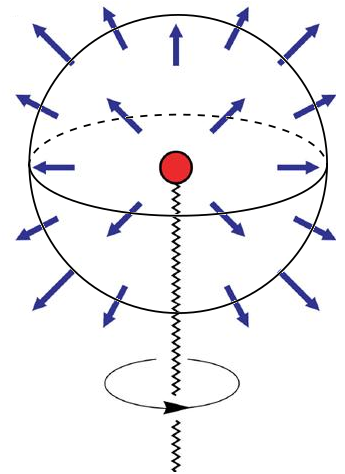
\includegraphics[scale=0.3]{DiracMon.png}
\caption{A schematization of Dirac string.}
\label{fig-DirMon}
\end{figure}

We call the two choices of $A$ respectively $A^+$ and $A^-$.
We say that $U_+ = \mathbb{R}^3 \setminus \qty{z<0}$ is the chart where we define $A^+$ and $U_- = \mathbb{R}^3 \setminus \qty{z>0}$ is the one where we define $A^-$.

Let us now show that the potentials indeed diverge near their Dirac string. We wish to integrate in a similar domain to the one of equation \eqref{eq:different-potentials}, however now we must exclude the Dirac string: the resulting domain is a 2D surface, which we denote by $S_2 \setminus D_\epsilon$; its boundary is a small circle $C_\epsilon$ around the Dirac string. As in \eqref{eq:MagnCharge} we have:
%
\begin{equation}\label{MagCharge}
g=\int_{S_2} F=\lim_{\epsilon\to 0}\int_{S_2\setminus D_{\varepsilon}}F=\lim_{\epsilon\to 0}\int_{S_2\setminus D_{\varepsilon}} \dd{A}=\lim_{\epsilon\to 0}\int_{C_{\varepsilon}} A,
\end{equation}
which implies the divergence of $A$, since its integral along an arbitrarily small circle is requested to be fixed and finite.

\medskip
We now want to calculate the transiton function between the two potentials in the region $U_+ \cap U_-$ where their domains overlap:
\begin{equation}
A^+-A^-=\frac{g}{2\pi}\dd{\phi}=\dd{\qty(\frac{g\phi}{2\pi})} \equiv \dd{\lambda(x)}\,.
\end{equation}

This transformation can be seen as a $U(1)$ gauge transformation:
let $h$ be the map $h:U_+\cap U_- \to G=U(1)$, such that $x\to \exp(ie\lambda(x))$, where $e$ is the electric charge.
The corresponding transformation of the potential is:
%
\begin{equation}
A^+=A^-+\dd{\lambda}=h^{-1}A^-h-\frac{i}{e}h \dd{h}\,.
\end{equation}

In order to have  the function $h$ well defined, we must have $h(g\phi) = h(g(\phi+ 2\pi))$.
This condition is satisfied if we assume that: 
\begin{equation}
ge \in 2\pi\mathbb{Z}.
\label{eq:Dirac}
\end{equation}
Expression  \eqref{eq:Dirac} is the so-called \textit{Dirac Quantization Condition} and guarantees that: 
\begin{equation}
h(g(\phi + 2\pi)) =  \exp(2 \pi ge)  h(g\phi) = h( g \phi) \,.
\end{equation}
We now want to show that the integer $eg$ has a clear geometrical meaning: it is the winding number of the map $h$, i.e. the number of times $h$ wraps around the circle $S^1$ as $x$ goes around the center once.
To prove this, we can split the integral in \eqref{MagCharge} into two contributions from both the potentials and integrate them over two hemispheres, whose borders can both be made to coincide with the equator $S^1$, but will have opposite orientations, whence the minus sign before $A_-$:

\begin{equation}
g=\int_{S^2}F=\int_{S^2_+}\dd{A}^++\int_{S^2_-}\dd{A}^-=\int_{S^1}\qty(A^+-A^-)=\int_{S^1}\dd{\lambda}=\Delta\lambda,
\end{equation}
%
Multiplying $\Delta \lambda$ by the charge $e$, we can deduce how many radiants the argument of the exponent has elapsed. Therefore, the winding number $S_1$ is: 
\begin{equation}
S_1=\frac{e\Delta\lambda}{2\pi}=\frac{ge}{2\pi} \,.
\end{equation}


\subsection{Zwanziger-Schwinger Quantization for the Dyon}
We want now to consider the hypothetical case of a particle carrying both electric and magnetic charge, respectively $e_1$ and $g_1$, which is called a dyon. If this particle moves into an electromagnetic field it experiences the force
\begin{equation}
\vec F=e_1\left[\vec E-\vec v\times\vec B\right]-g_1\left[\vec B-\vec v\times\vec E\right].
\end{equation}

At the same time we suppose that electric and magnetic fields are origined by another dyon in the origin, with electric charge $e_2$ and magnetic charge $g_2$, which generates the fields:
\begin{align}
&\vec E=\frac{e_2}{4\pi}\frac{\vec r}{r^3},\nonumber\\
&\vec B=\frac{g_2}{4\pi}\frac{\vec r}{r^3}.
\end{align}

Now, let $\vec L=\vec r\times m\vec v$ (where $m$ denotes the mass) be the orbital angular momentum of the first dyon: in this case we have
\begin{equation}
\dv{\vec{L}}{t}
=\frac{1}{4\pi}(e_1g_2-g_1e_2)
\dv{}{t}
\frac{\vec r}{r},
\end{equation}
which implies that a dyon in this field does not conserve the regular angular momentum $\vec L$, however it conserves another quantity, which we denote by $\vec{J}$:
\begin{equation}
\vec J=\vec r\times m\vec v-\frac{1}{4\pi}(e_1g_2-g_1e_2)\frac{\vec r}{r}.
\end{equation}
Consider now the projection of $\vec J$ on the versor $\hat r$, which is $J_r=(e_1g_2-g_1e_2)/4 \pi$: from the quantization of $J_r$: $J_r \in \mathbb Z /2 $, the Zwanziger-Schwinger quantization condition follows:
\begin{equation}
e_1g_2-g_1e_2\in 2 \pi \mathbb{Z}.
\end{equation}
We notice that if we set $g_1=0$, $e_2=0$ and $e_1 = e$, that is, we consider an electrically charged particle with unit charge moving in the field generated by a pure magnetic monopole, we get Dirac's quantization condition:
\begin{equation}
e g_2\in 2 \pi \mathbb{Z}.
\end{equation}

% \subsection{Witten Effect}
% Now we want to generalize quantization that are deduced from a generic gauge transformation about a direction $\vec\phi$. In this case we have that variations of a generic isovector $\vec v$ and vector potential $\vec A_\mu$ are
% \begin{subequations}
% \begin{align}
% &\delta\vec v=\frac{\vec\phi\times\vec v}{a}\\
% &\delta\vec A_\mu=-\frac{D_\mu\vec\phi}{ea},
% \end{align}
% \end{subequations}

% where we have the normalization constant $a$, the electric charge $e$ and where we defined the covariant derivative
% \begin{equation}
% D_\mu\vec\phi=\partial_\mu\vec\phi-e\vec A_\mu\times\vec\phi.
% \end{equation}
% Considering now the operator $e^{2\pi i N}$, where $N$ is the same operator with Higgs solution that will be defined in the next section. In the vacuum $D_\mu\vec\phi=0$ and at infinity in space we have that this operator is equal to identity. Using the variations defined above, we can obtain the Noether charge of the related transformations, which is for $\delta\vec\phi=0$
% \begin{equation}
% N=-\int_{\mathbb{R}^3}\frac{1}{ae}\frac{\partial\mathcal{L}}{\partial\partial_0\vec A_i}\cdot D_i\phi=\frac{q}{e},
% \end{equation}
% where we used the fact that the conjugated momentum of $\vec A_i$ is $-\vec E_i$.
% Instead, if we add a new term in the action
% \begin{equation}
% \mathcal{L}_\theta=\frac{e^2\theta}{64\pi^2}\epsilon^{\alpha\beta\mu\nu}\vec G_{\alpha\beta}\vec G_{\mu\nu},
% \end{equation}
% where $\vec G^{\alpha\beta}$ are the gauge field-strengths for $A$. In this case we have a modify of $N$ by a factor
% \begin{equation}
% \Delta N=-\frac{e\theta}{16\pi^2a}\int_{\mathbb{R}^3}\epsilon^{0i\alpha\beta}\vec G_{\alpha\beta}D_i\vec\phi=\frac{e\theta g}{8\pi^2},
% \end{equation}
% with the magnetic charge $g$. Rewriting this expression it follows, for $eg=-4\pi$ (the t' Hooft-Polyakov monopole result, which will be obtained later)\begin{equation}
% q=ne+\frac{e\theta}{2\pi},
% \end{equation}
% with $n\in\mathbb{Z}$. This is the generalization to have consistency with quantization condition, a result by Edward Witten \cite{Witten}.
\end{document}